\documentclass[]{article}
\usepackage{lmodern}
\usepackage{amssymb,amsmath}
\usepackage{ifxetex,ifluatex}


\usepackage[utf8]{inputenc}
\usepackage[english,russian,ukrainian]{babel}

\usepackage{fixltx2e} % provides \textsubscript
\ifnum 0\ifxetex 1\fi\ifluatex 1\fi=0 % if pdftex
  \usepackage[T1]{fontenc}
  \usepackage[utf8]{inputenc}
\else % if luatex or xelatex
  \ifxetex
    \usepackage{mathspec}
  \else
    \usepackage{fontspec}
  \fi
  \defaultfontfeatures{Ligatures=TeX,Scale=MatchLowercase}
\fi
% use upquote if available, for straight quotes in verbatim environments
\IfFileExists{upquote.sty}{\usepackage{upquote}}{}
% use microtype if available
\IfFileExists{microtype.sty}{%
\usepackage{microtype}
\UseMicrotypeSet[protrusion]{basicmath} % disable protrusion for tt fonts
}{}
\usepackage[unicode=true]{hyperref}
\hypersetup{
            pdfborder={0 0 0},
            breaklinks=true}
\urlstyle{same}  % don't use monospace font for urls
\usepackage{graphicx,grffile}
\makeatletter
\def\maxwidth{\ifdim\Gin@nat@width>\linewidth\linewidth\else\Gin@nat@width\fi}
\def\maxheight{\ifdim\Gin@nat@height>\textheight\textheight\else\Gin@nat@height\fi}
\makeatother
% Scale images if necessary, so that they will not overflow the page
% margins by default, and it is still possible to overwrite the defaults
% using explicit options in \includegraphics[width, height, ...]{}
\setkeys{Gin}{width=\maxwidth,height=\maxheight,keepaspectratio}
\IfFileExists{parskip.sty}{%
\usepackage{parskip}
}{% else
\setlength{\parindent}{0pt}
\setlength{\parskip}{6pt plus 2pt minus 1pt}
}
\setlength{\emergencystretch}{3em}  % prevent overfull lines
\providecommand{\tightlist}{%
  \setlength{\itemsep}{0pt}\setlength{\parskip}{0pt}}
\setcounter{secnumdepth}{0}
% Redefines (sub)paragraphs to behave more like sections
\ifx\paragraph\undefined\else
\let\oldparagraph\paragraph
\renewcommand{\paragraph}[1]{\oldparagraph{#1}\mbox{}}
\fi
\ifx\subparagraph\undefined\else
\let\oldsubparagraph\subparagraph
\renewcommand{\subparagraph}[1]{\oldsubparagraph{#1}\mbox{}}
\fi

\date{}


\usepackage{enumitem}
\makeatletter
\newcommand{\xslalph}[1]{\expandafter\@xslalph\csname c@#1\endcsname}
\newcommand{\@xslalph}[1]{%
    \ifcase#1\or а\or б\or в\or г\or д\or e\or є\or ж\or з\or i%
    \or й\or к\or л\or м\or н\or о\or п\or р\or с\or т%
    \or у\or ф\or х\or ц\or ч\or ш\or ю\or я\or аа\or бб\or вв%
    \else\@ctrerr\fi%
}
\AddEnumerateCounter{\xslalph}{\@xslalph}{m}
\makeatother

\graphicspath{ {./ }}

\begin{document}


\newpage
\subsection{ 7. Статичні масиви. Багатовимірні масиви }
\setcounter{subsection}{1}

Задачі для аудиторної роботи

\begin{enumerate}
\def\labelenumi{\arabic{enumi})}
\item
  Двовимірна матриця 3х3 ініціалізована числами
  \{\{1,2,3,\},\{4,5,6\},\{7,8,9\}\}. Транспонуйте цю матрицю, введіть
  натуральні числа N і M та замініть елемент, що рівний числу M (якщо
  він є в матриці на число N. Виведіть отриману матрицю рядок за
  рядком.
\item
  Двовимірна матриця 3х3 ініціалізована дійсними числами \{\{1.0,
  2,3,\},\{4,5,6\},\{7,8,9\}\}. Транспонуйте цю матрицю, введіть
  натуральні числа I і J та дійсне число A замініть елемент з індексами
  IJ на число A (відслідкуйте при цьому коректність індексів). Виведіть
  отриману матрицю рядок за рядком.
\item
  Напишіть функцію для вводу двовимірної дійсної матриці довільного
  розміру m x n, яка вводить з підказкою для користувача (вказуючи
  індекси елементів) кожен елемент в одному рядку. Величини m, n
  вводяться з консолі та їх значення менші за 20.
\item
  Напишіть функцію для вводу двовимірної цілої (дійсної) матриці
  довільного розміру m x n, яка вводить з підказкою для користувача
  (номер рядку) матрицю рядок за рядком (числа в рядку розділяються
  одним пробілом). Величини m, n вводяться з консолі та їх значення
  менші за 25.
\item
  В двовимірному масиві A{[}N,M{]} знайдіть суму елементів A{[}i,j{]},
  що $i-j=k$. Ціле число $k$ може бути від'ємним, якщо таких елементів
  немає, то вивести нуль. Величини $M, N$ вводяться з консолі та їх
  значення менші за 100.
\end{enumerate}

Задачі для самостійної роботи

\begin{enumerate}
\def\labelenumi{\arabic{enumi})}
\item
  Дана матриця розміру $n \times m$. Поміняти місцями її стовпці так, щоб їх
  максимальні елементи утворювали спадаючу послідовність.
\item
  Знайдіть квадратну матрицю, зворотну даної з розміром $n \times n$.
\item
  Дана квадратна матриця порядку $2n$. Повернути її на 180 градусів в
  позитивному напрямку.
 \newpage
\item
  Заповнити двовимірний квадратний масив $n\times n$ цілими числами від 1 до $n^2$ по
  спіралі, як показано на наступному малюнку:\\
  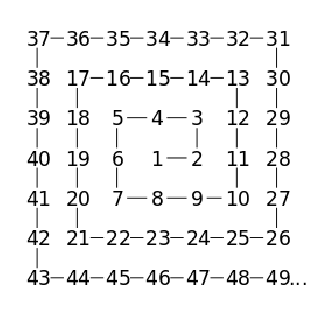
\includegraphics{spiral5}
   
\item
  Дана матриця розміру $n \times m$. Поміняти місцями стовпці, що містять
  мінімальний і максимальний елементи матриці.
\item
  Дано дві матриці $n \times m$ і $m \times k$. Отримайте їх добуток.
\item
  Дана матриця розміру $n \times m$. Поміняти місцями її рядки так, щоб їх
  максимальні елементи утворювали зростаючу послідовність.
\item
  У даній дійсної квадратної матриці порядку $n$ знайти найбільший по
  модулю елемент.
\item
  Отримати квадратну матрицю порядку $n - 1$ шляхом викидання з вихідної
  матриці будь-якого рядка і стовпця, на перетині яких розташований
  елемент зі знайденим значенням. Виконуйте до тих пір, поки не
  залишиться останній елемент.
\item
  Дана квадратна матриця порядку $2n + 1$. Дзеркально відобразити її
  елементи відносно побічної діагоналі матриці.
\item
  Дана дійсна квадратна матриця порядку $2n + 1$. Отримати нову матрицю,
  повернувши її блоки, обмежені діагоналями, на 90 градусів.
\item
  Дана матриця розміру $n \times m$. Поміняти місцями її перший і останній
  рядки, що містять тільки негативні елементи.
\item
  Дана цілочисельна матриця розміру $n \times m$. Знайти елемент, який є
  максимальним у своєму рядку і мінімальним в своєму стовпці. Якщо такий
  елемент відсутній, то вивести 0.
\item
  Складіть програму циклічної перестановки стовпців двовимірного масиву
  $n \times m$, при якій зсуві зсувається вправо на $k$ стовпців.
\item
  Дана матриця розміру $n \times m$. Поміняти місцями її стовпці так, щоб їх
  мінімальні елементи утворювали зростаючу послідовність.
\item
  Дана квадратна матриця порядку $2n + 1$. Дзеркально відобразити її
  елементи відносно вертикальної осі симетрії матриці.
\item
  Дана квадратна матриця порядку $2n$. Повернути її на 270 градусів в
  позитивному напрямку щодо її центру.
\item
  Дана матриця розміру $n \times m$. Поміняти місцями рядки, що містять
  мінімальний і максимальний елементи матриці.
\item
  У квадратній таблиці обміняйте місцями елементи рядка і стовпця, на
  перетині яких знаходиться мінімальний з позитивних елементів.
\item
  Дана квадратна матриця порядку $2n$. Повернути її на 90 градусів в
  позитивному напрямку щодо її центру.
\item
  Дана квадратна матриця порядку $2n + 1$. Дзеркально відобразити її
  елементи відносно головної діагоналі матриці.
\item
  Складіть програму циклічної перестановки рядків двовимірного масиву $n \times m$,
  при якій зсув відбувається вниз на $k$ рядків.
\item
  Дана матриця розміру $n \times m$. Поміняти місцями її перший і останній
  стовпці, що містять тільки позитивні елементи.
\item
  Заповнити двовимірний квадратний масив цілими числами від 1 до 100 по
  спіралі, починаючи від центру і закручуючи за годинниковою стрілкою.
\item
  Заповніть квадратну матрицю $n \times n$ за принципом латинського квадрата: в
  кожному рядку і кожному стовпці використовуються лише числа від 1 до n
  що не повторюються між собою.
\item
  Дана матриця дійсних коефіцієнтів. Впорядкувати її рядки по неспаданню
  перших елементів, суми значень рядків, величині найменших елементів
  рядків.
\end{enumerate}

Додаткові задачі:

\begin{enumerate}
\def\labelenumi{\arabic{enumi})}
\item
  Дана матриця $n \times m$ з нулів та одиниць. Знайти найбільший за площиною
  прямокутник з одних одиниць. Зробіть цю задачу без вкладених 4-х
  циклів для $0<n,m<255$.
\end{enumerate}


\end{document}
